\chapter{메인 스레드와 Handler}
메인 스레드에서 UI 이벤트를 처리하는 메커니즘을 살펴보자. Handler는 메인 Looper와 연결되어 메인 스레드에서 Message를 처리하는 중심 역할을 한다. Handler는 백그라운드 스레드에서도 특별한 용도로 사용 가능하다는 점에서 다음 장의 백그라운드 스레드와도 내용이 연결된다.

\section{메인 스레드}
애플리케이션 동작은 당연히 멀티 스레드이지만, UI를 업데이트하는 데는 단일 스레드 모델(Single Thread Model: 해당 변수나 메서드를 사용하는 시점에는 하나의 스레드만 실행)이 적용된다.\footnote{롤리팝에서는 Render Thread가 추가되어 offload atomic animation을 실행한다}
멀티 스레드로 UI를 업데이트하면 동일한 UI 자원을 사용 시 교착 상태(deadlock), 경합 상태(race condition) 등 여러 문제가 발생하기 때문에 메인 스레드에서만 UI 업데이트를 허용하고 있다.\\
% 싱글 스레드 이벤트 큐 모델

\begin{comment}
\colorbox{tearose}{\parbox[t]{15cm}{
스레드 A가 특정 lock을 잡고 있으면 그 lock을 확보해야 하는 다른 스레드 B에서는 대기해야 한다. 그런데 B에서는 A에서 추가로 확보하려고 하는 lock을 이미 잡고 있다면, 서로 lock이 풀릴 때까지 계속 대기할 수 밖에 없다. 이것이 교착 상태이다. 
예를 들어 화면에 성과 이름을 입력하려는 A, B 두 스레드가 있다. 
두 스레드는 자신이 입력한 것이 바로 덮어 쓰여지는 것이 싫고, 온전히 이름을 다 입력하고자 한다. 
그래서 한국인 이름을 입력하는 A 스레드에서는 다른 스레드가 접근 못하도록 lock을 잡고서 입력하고서, 그 다음에 이름을 입력하려고 한다.
외국인 이름을 입력하는 스레드에서는 이름에 접근하면서 lock을 잡고, 그 다음에 성에 접근하려고 한다. 이 때 두 스레드는 어느 시점에 교착 상태에 이르게 된다. 교착 상태는 일반적으로 lock을 잡는 순서를 일정하게 하면 해결되지만, 복잡한 프로그램에서 이 순서를 맞추는 게 간단치 않고 성능에 나쁜 영향을 줄 수도 있다.\footnote{\url{https://ko.wikipedia.org/wiki/교착_상태}를 참고하자.}\\
경합 상태는 2개 이상의 스레드에서 공유 데이터에 접근해서 동시에 변경하려 할 때 발생한다. 스레드 실행은 내부적으로 스레드 스케줄링 알고리즘에 따르기 때문에, 스레드끼리 어느 것이 먼저 공유 데이터에 접근할지 순서는 알 수 없고 스레드끼리 경주(racing)하는 상황이 생긴다.\\

러브 액츄얼리라는 영화에서 많이 기억되는 장면이 있는데, 사랑하는 상대방한테 남자가 창밖에서 종이를 한 장씩 넘기며 고백하는 장면이다.
비유하자면 이것이 바로 안드로이드에서 UI를 업데이트 하는 방식이다. 상대방에게 보여주는 종이가 바로 UI 화면이라고 보면 된다. 종이가 스케치북으로 되어 있어 순서대로 넘기는 것은 일종의 순서를 보장하는 큐라고 할 수 있다. 그리고 종이를 넘기는 남자는 메인 스레드에 해당한다.
만일 남자(메인 스레드)가 혼자서 종이를 넘기지 않고, 다른 사람(스레드)에게 종이를 상대방이 보는 화면 앞으로 종이를 가져오라고 하면, 어떤 일이 벌어질까? 바로 이 상황이 경합 상태이다. 종이의 순서를 보장할 수 없으니 사랑 고백이 엉뚱한 얘기가 될 수도 있고, 어느 종이는 순식간에 다른 종이로 바뀔 테니, 상대방이 못 보는 메시지도 생겨난다.
}}\newline\newline
\end{comment}

앱이 시작되면서 메인 스레드가 생성된다. 컴포넌트는(Activity, Service, BroadcastReceiver, Application) 메인 스레드에서 시작되고 그 안의 메서드 호출은 기본적으로 메인 스레드에서 실행된다. 
메인 스레드는 UI를 변경할 수 있는 유일한 방법이기 때문에 메인 스레드를 UI 스레드라고 부르기도 한다. 
Service, BroadcastReceiver, Application은 직접적으로 UI는 아니기 때문에, UI 스레드라는 것은 메인 스레드의 한 부분만을 얘기하는 것이지만 이해를 위해 많이 사용된다.\\

일반적인 자바 애플리케이션에서는 main() 메서드로 실행되는 것이 바로 메인 스레드이다.
\begin{lstlisting}[frame=single] 
public class Hello {

	public static void main(String[] args) {
		System.out.print("Hello");
	}

}
\end{lstlisting}

안드로이드 애플리케이션의 메인 스레드는 뭔가 다른 특별한 것일까? 그렇지 않다. 
안드로이드 프레임워크 내부 클래스인 android.app.ActivityThread가 바로 애플리케이션의 메인 클래스\footnote{실제로는 ZygoteInit이 시작점이지만 우리가 이해해야 하는 지점은 ActivityThread부터이다.}이고, ActivityThread의 main() 메서드가 애플리케이션의 시작 지점이다.
\begin{lstlisting}[frame=single, caption=ActivityThread.java] 
	public static void main(String[] args) {
		SamplingProfilerIntegration.start();

		CloseGuard.setEnabled(false);

		Environment.initForCurrentUser();

		EventLogger.setReporter(new EventLoggingReporter());

		Process.setArgV0("<pre-initialized>");

		Looper.prepareMainLooper();

		ActivityThread thread = new ActivityThread();
		thread.attach(false);

		if (sMainThreadHandler == null) {
			sMainThreadHandler = thread.getHandler();
		}

		AsyncTask.init();

		if (false) {
			Looper.myLooper().setMessageLogging(
					new LogPrinter(Log.DEBUG, "ActivityThread"));
		}

		Looper.loop(); // (1)

		throw new RuntimeException("Main thread loop unexpectedly exited");
	}
\end{lstlisting}

여기서 제일 중요한 곳은 28라인(1)이다. 
Looper.loop() 메서드에는 무한반복문이 있어서 main() 메서드는 프로세스가 종료될 때까지 끝나지 않는다.
ActivityThread는 클래스명 때문에 Thread를 상속한 게 아닐까 하는 오해를 받기도 하지만 전혀 그렇지 않다.
게다가 Activity만 관련돼 있는 것도 아니고 모든 컴포넌트들이 다 관련돼 있다.

%http://warmz.tistory.com/588
% http://www.myexception.cn/android/1710667.html
% http://www.2cto.com/kf/201407/317129.html

\section{Looper}
Looper 클래스\footnote{\url{http://developer.android.com/reference/android/os/Looper.html}}는 내용이 단순하다. Looper에서 필요한 내용을 알아보자.
\begin{itemize}
\item TLS(Thread Local Storage)에 Looper를 넣는다. 구체적으로 ThreadLocal<Looper>에 set() 메서드로 새로운 Looper를 추가하고 get() 메서드로 Looper를 가져오는데, 각 스레드별로 다른 Looper가 반환된다.
Looper.prepare()를 통해 스레드별로 Looper를 생성하고, 특히 메인 스레드의 Looper는 ActivityThread에서 Looper.prepareMainLooper()를 통해서 생성되고, Looper.getMainLooper()를 통해서 어디서든 가져올 
수 있다.
\item Looper별로 MessageQueue를 가진다. 특히 메인 스레드에서는 이 MessageQueue를 통해서 UI 작업에서 경합 상태를 해결한다. 
개발 중에 Queue 구조가 필요할 때 java.util.Queue의 여러 구현체를 사용할 수도 있지만 Looper 사용도 고려해보자. 특히 스레드별로 다른 Queue를 사용할 때는 Looper를 사용하는 게 더 단순해질 수 있다.(결론적으로는 Handler를 사용하는 것이다.)
\end{itemize}

Looper.loop() 메서드의 주요 코드를 보자.
\begin{lstlisting}[frame=single, caption=Looper.java] 
	public static void loop() {
		final Looper me = myLooper();
		if (me == null) {
			throw new RuntimeException(
					"No Looper; Looper.prepare() wasn't called on this thread.");
		}
		final MessageQueue queue = me.mQueue;
		for (;;) {
			Message msg = queue.next(); // (1)
			if (msg == null) {
				return; // (2)
			}
			msg.target.dispatchMessage(msg); // (3)
			msg.recycle();
		}
	}
	
	public void quit() {
        mQueue.quit(false);
    }
    
    public void quitSafely() {
        mQueue.quit(true);
    }
\end{lstlisting}	
\begin{itemize}
\item 13라인(1)이 바로 메시지를 처리하는 부분이다. 
for 루프를 돌면서 MessageQueue에서 다음 메시지를 꺼내서 13라인(3)에서 dispatchMessage()를 호출한다. 
\item quit(), quitSafely() 메서드는 Looper를 종료한다. 구체적으로 MessageQueue의 quit() 메서드에 boolean 값을 전달하고, 9라인(1)의 queue.next()에서 null을 리턴하고 11라인(2)에서 for 루프가 종료된다.
Looper API 문서에서 quit()과 quitSafely() 메서드 차이를 보도록 하자.
quit() 메서드는 아직 처리되지 않은 Message는 모두 제거한다.
quitSafely() 메서드는 sendMessageDelayed() 등을 써서 실행 시간을 뒤로 미룬 경우에 해당하는 것으로, quitSafely() 메서드를 실행하는 시점에 현재 시간보다 뒤쪽에 있는 Message를 제거하고 그 앞쪽에 있는 Message는 계속해서 처리를 진행한다. 다만 quitSafely() 메서드는 젤리빈 API 레벨 18 이상에서 쓸 수 있다.\\
\end{itemize}

\section{Message와 MessageQueue}
\label{sec:messagequeue}
MessageQueue는 Message를 담고 있는 자료구조이다.
MessageQueue의 구조는 ArrayBlockingQueue보다는 LinkedBlockingQueue에 가깝다. ArrayBlockingQueue는 배열에 노드를 추가하는 방식이지만, LinkedBlockingQueue는 다음 노드에 대한 링크를 변수로 가진다. 
Array 구조에 비해서 Link 구조는 일반적으로 개수의 한계가 없고 삽입 속도가 빠르다. 
대신 Array 구조는 랜덤 인덱스 접근이 가능하고 Link 구조는 순차 접근을 해야 한다. MessageQueue는 실행하기로 한 시간 순으로 삽입되어서 빠른 것부터 순차적으로 꺼내어진다.\\

먼저 Message 클래스를 보자.
\begin{lstlisting}[frame=single, caption=Message.java] 
public final class Message implements Parcelable {

	public int what;

	public int arg1;

	public int arg2;

	public Object obj;

	public Messenger replyTo;
	
	....

	/* package */long when;

	/* package */Bundle data;

	/* package */Handler target;

	/* package */Runnable callback;

	/* package */Message next;
	
	....
}
\end{lstlisting}
MessageQueue에 들어가는 android.os.Message에는 public 변수에 int arg1, int arg2, Object obj,
Messenger replyTo, int what 5개가 있고 Message를 만들 때 이 변수에 값을 넣는다.
Message에는 package private 변수도 여러 개 있다. android.os 패키지 아래에 Looper, Message, MessageQueue, Handler가 모두 있어서, 이들 클래스에서 Message의 package private 변수에 직접 접근한다. target이나 callback 같은 것들이 Handler에서 postXxx(), sendXxx() 메서드를 호출할 때 Message에 담겨서 MessageQueue에 들어간다. postXxx(), sendXxx() 메서드에서 실행하려는 시간(AtTime)이 전달되고, 나중에 호출한 것이라도 AtTime이 앞서면 Queue 중간에 삽입된다. 이것이 삽입이 쉬운 Link 구조를 사용한 이유이다.\\

Message를 생성할 때는 오브젝트 풀(object pool)에서 가져오는 Message.obtain() 메서드나 Handler의 obtainMessage() 메서드를 사용하는 것을 권장한다. 내부적으로 Handler의 obtainMessage()는  Message.obtain()을 다시 호출한다.
오브젝트 풀은 Message에 정적 변수로 있고(여기서도 Link로 연결됨) 최대 50개까지 Message를 저장한다. 그리고 Looper.loop() 메서드에서 Message를 처리하고 나서 recycleUnChecked() 메서드를 통해 Message를 초기화하고 최대 개수에 도달하지 않았다면 오브젝트 풀에 추가하는 형태이다.
new Message()와 같이 기본 생성자를 가지고서 값을 채워도 동작에는 문제가 없어 보이지만, Message 처리가 끝나면 불필요하게 풀에 추가하는 동작이 되어서 최대 개수에 이르는 건 시간 문제가 된다. 
풀에서 가져와서(여분이 없으면 새로 생성) 풀에 돌려줘야지 따로 생성해서 풀에 돌려주는 건 불필요한 자원 낭비가 된다.\footnote{Handler를 통해 Message를 처리하는 게 아니라, 파라미터에 별도 객체를 전달하지 않고 Message를 대신 사용해서 주고받는 경우에만 Message 기본 생성자로 쓰도록 하자.}\\

%Handler의 removeMessages 메서드에서는 원하는 Message를 제거하기 위해 Queue를 순회하는데, 이 경우에는 Link 구조가 조금 불리해진다.

\section{Handler}
Handler는 Message를 MessageQueue에 넣는 기능과 MessageQueue에서 꺼내 처리하는 기능을 함께 제공한다. Handler와 Looper, MessageQueue의 관계, 그리고 사용 방법에 대해서 알아보자.

\subsection{Handler 생성}
Handler를 사용하려면 먼저 생성자를 이해해야 한다. 
Handler에는 기본 생성자 외에 Hanlder.Callback 또는 Looper가 전달되는 생성자들이 있다. 
당연한 얘기지만 내부적으로 파라미터가 가장 많은 4번째 생성자를 다른 생성자에서 호출한다.
\begin{itemize}
\item Handler()
\item Handler(Handler.Callback callback)
\item Handler(Looper looper)
\item Handler(Looper looper, Handler.Callback callback)
\end{itemize}

Handler는 Looper(결국 MessageQueue)와 연결되어 있는데, 이들 생성자와 어떤 관계일까? 기본 생성자는 바로 현재 스레드의 Looper를 사용하겠다는 의미이다.(Looper는 Thread Local Storage에 들어간다고 앞에서 얘기했다.)
Handler 기본 생성자를 메인 스레드에서 사용한다면, 이미 ActivityThread에서 메인 Looper를 생성했기 때문에 메인 Looper를 사용하는 것이다. 이것이 우리가 만드는 코드에서 가장 많이 사용하는 방식이다.\\

그럼 백그라운드 스레드에서 기본 생성자를 사용한다면 어떨까? 이때는 Looper가 준비되어 있지 않다면 RuntimeException을 발생시킨다. 
``Can't create handler inside thread that has not called Looper.prepare''
이 메시지에 따르면 먼저 Looper.prepare()를 실행해서 해당 스레드에서 사용할 Looper를 준비해야 한다.(내부적으로 prepare() 메서드는 MessageQueue를 생성하는 것 말고는 별 게 없다.)\\

Looper API 문서를 보면 백그라운드 스레드에서 Handler를 사용하는 방법이 나온다.

\begin{lstlisting}[frame=single, caption=LooperThead, label=src:LooperThread] 
class LooperThread extends Thread {
	public Handler mHandler;

	public void run() {
		Looper.prepare();

		mHandler = new Handler() {
        		public void handleMessage(Message msg) {
            		// process incoming messages here
			}
		};

		Looper.loop();
	}
}
\end{lstlisting}
LooperThread에서 스레드를 시작하면 Looper.loop()에 무한 반복문이 있기 때문에 해당 스레드는 종료되지 않고, mHandler에서 sendXxx(), postXxx() 메서드를 사용하면 스레드 내에서 handleMessage() 메서드를 실행한다.\\

그런데 앱을 만들다 보면 가끔 위에 얘기한 RuntimeException을 만나는 경우가 있다.
예를 들어, 어떤 메서드가 단순하게 TextView의 setText()를 실행하는 것이지만, 이 내용이 메서드 콜을 하는 곳이 여러 군데이거나 메서드 콜 스택이 깊어서 어디서 호출하는지 금방 파악이 안 되는 경우도 있다.
여러 곳에서 사용하는 메서드라면 메인 스레드뿐 아니라 백그라운드 스레드에서도 호출할 가능성이 있다. 
new Handler()로 생성하고 post() 메서드를 통해서 TextView를 변경하려 하는데, Handler 생성을 메인 스레드에서 하는지 백그라운드 스레드에서 하는지 모호한 경우가 있다.
메인 스레드라면 이미 메인 Looper가 있는데 백그라운드 스레드라면 대응하는 Looper가 당장 없을 때 RuntimeException을 만나게 된다.\\

예를 들어, 아래 코드에서는 BadgeListener의 updateBadgeCount()에서 UI를 변경한다.
\begin{lstlisting}[frame=single] 
	public void process(BadgeListener listener) {
		int count = ...
		listener.updateBadgeCount(count);
	}
\end{lstlisting}	

process() 메서드는 메인 스레드에서 호출한다면 문제가 없지만, 백그라운드 스레드에서 호출할 때 CalledFromWrongThreadException을 발생시킨다. 
이때 Looper와 Handler의 관계를 잘 모른다면 아래처럼 작성할 수 있다.
\begin{lstlisting}[frame=single] 
	public void process(BadgeListener listner) {
		int count = ...
		new Handler().post(new Runnable() {
		
			public void run() {
				listner.updateBadgeCount(count);
			}
			
		});
	}
\end{lstlisting}	
백그라운드 스레드에서는 Looper가 연결되어 있지 않다면 RuntimeException이 발생한다.
UI 업데이트이기 때문에 백그라운드 스레드의 Looper를 생성해도 도움이 안 되고, 바로 메인 Looper를 사용해야 한다. 메인 Looper와 연결된 Handler를 사용하는 것으로 Handler의 여러 생성자 가운데 세 번째 생성자를 사용하면 된다.
\begin{lstlisting}[frame=single] 
	public void process(BadgeListener listner) {
		int count = ...
		new Handler(Looper.getMainLooper()).post(new Runnable() {
		
			public void run() {
				listner.updateBadgeCount(count);
			}
			
		});
	}
\end{lstlisting}

\subsection{Handler 동작}
Handler는 Message를 MessageQueue에 보내는 것과 Message를 처리하는 것을 함께 제공한다. post(), postAtTime(), postDelayed() 메서드를 통해서 Runnable 객체도 전달되는데, 실제로 Runnable도 내부적으로 Message에 포함되는 값이다.\\

Handler에서 Message를 보내는 메서드 목록을 살펴보자.\\

\scalebox{0.8}{
\begin{tabular}[fontsize=\tiny]{|l|l|l|} \hline
 & send & post \\ \hline
기본 & sendEmptyMessage(int what) & post(Runnable r)
\\
 & sendMessage(Message msg) & \\ \hline
Delayed & sendEmptyMessageDelayed(int what, long delayMillis) & postDelayed(Runnable r, long delayMillis)\\
 & sendMessageDelayed(Message msg, long delayMillis) & \\ \hline
AtTime & sendEmptyMessageAtTime(int what, long uptimeMillis)
 & postAtTime(Runnable r, Object token, long uptimeMillis) \\
  & sendMessageAtTime(Message msg, long uptimeMillis) & postAtTime(Runnable r, long uptimeMillis)\\ \hline
FrontOfQueue & sendMessageAtFrontOfQueue(Message msg)
 & postAtFrontOfQueue(Runnable r)
\\ \hline
\end{tabular}
}
\newline

\begin{itemize}
\item Message의 what 값만을 전달하는 sendEmptyMessage(), sendEmptyMessageDelayed(), sendEmptyMessageAtTime() 메서드가 있다.
\item -Delayed로 끝나는 메서드는 내부적으로 -AtTime 메서드를 호출한다. 현재 uptimeMillis에 delayMillis를 더한 값이 uptimeMillis 파라미터에 들어간다.
\item postAtFrontOfQueue() 메서드는 특별한 상황이 아니면 쓰지 말라는 가이드가 있다. 
권한 문제나 서버 문제와 같이 앱을 더 이상 사용할 수 없는 특별한 때가 아니면 사용할 일이 없다. 남용하면 안 되는 메서드이다.
\end{itemize}

Looper.loop() 메서드에서 호출하는 Handler의 dispatchMessage() 메서드를 보자.
\begin{lstlisting}[frame=single, caption=Handler.java] 
	public void dispatchMessage(Message msg) {
		if (msg.callback != null) { // (1)
			handleCallback(msg);
		} else {
			if (mCallback != null) {
				if (mCallback.handleMessage(msg)) {
					return;
				}
			}
			handleMessage(msg);
		}
	}
	
	private static void handleCallback(Message message) {
		message.callback.run();
	}
\end{lstlisting}
dispatchMessage()는 public 메서드이다. 
드물긴 하지만 sendXxx()나 postXxx() 메서드를 쓰지 않고 직접 dispatchMessage() 메서드를 사용하기도 하는데, 이때는 MessageQueue를 거치지 않고 직접 메시지를 처리하는 것이다.
2라인(1)에서 callback Runnable이 있다면 그것을 실행하고 아니면 handleMessage()를 호출하고 있다.

\subsection{Handler 용도}
Handler는 일반적으로 UI 갱신을 위해 사용된다. 관련해서 해당 케이스를 살펴보자.
\begin{itemize}
\item 네트워크나 DB 작업 등 스레드 작업 중에 UI를 업데이트한다. 
AsyncTask에서도 내부적으로 Handler를 이용해서 onPostExecute() 메서드를 실행한다.
\item UI 작업 중에 다음 UI 갱신 작업을 MessageQueue에 넣어 예약한다. 작업 예약이 필요한 경우가 있다.
예를 들어, Activity의 onCreate() 메서드에서 하지 못하는 여러 가지 일들이 있다. 소프트 키보드를 띄운다든가, ListView의 setSelection() 메서드를 호출한다든가 하는 것이 onCreate() 메서드에서는 잘 동작하지 않는다. 이때 Handler를 이용해서 현재 작업이 끝난 이후에 다음 타이밍을 기다려서 진행한다.
\item 반복적으로 UI를 갱신한다. DigitalClock이나 TextClock 같은 위젯도 Handler를 이용해서 현재 시간을 갱신하고 있다.
반복적인 UI 갱신 패턴은 아래와 같다.
\begin{lstlisting}[frame=single] 
  	private static final int DELAY_TIME = 2000;
	private Runnable updateTimeTask = new Runnable() {

		@Override
		public void run() {
			systemInfo.setText(monitorService.getSystemInfo());
			...
			handler.postDelayed(this, DELAY_TIME); // (1)
		}

	};
	
	public void onClickButton(View view) {
		handler.post(updateTimeTask); 
	}
\end{lstlisting}
UI 갱신이 끝나고 8라인(1)에서 postDelayed()에 Runnable 자체를 전달해서 계속 반복하게 된다.
\item 시간을 제한할 때 사용한다. 안드로이드 내부적으로 ANR을 판단할 때도 사용하는 방법이다.
아래 코드는 개발자 가이드에 있는 것인데, 블루투스 LE 디바이스를 스캔할 때 시간 제한을 둔 것이다.
\begin{lstlisting}[frame=single] 
	private static final long SCAN_PERIOD = 10000;
	...
	private void scanLeDevice(final boolean enable) {
	    if (enable) {
	    	mHandler.postDelayed(new Runnable() { // (1)
	    		
	    		@Override
	    		public void run() {
	    			mScanning = false;
	    			mBluetoothAdapter.stopLeScan(mLeScanCallback);
	    		}
	    	}, SCAN_PERIOD);
	
	    	mScanning = true;
	    	mBluetoothAdapter.startLeScan(mLeScanCallback); // (2)
	    } else {
	    	mScanning = false;
	    	mBluetoothAdapter.stopLeScan(mLeScanCallback);
	    }
	    ...
	}
\end{lstlisting}
15라인(2)에서 startLeScan()을 실행하는데, 5라인(1)의 postDelayed(Runnable) 메서드에서 10초 후에 stopLeScan()을 실행하도록 Runnable Message를 전달하였다.\\

앱에서 많이 사용하는 방식으로 몇 초 내에 Back 키를 다시 누를 때만 종료하게 할 때도 마찬가지 방식을 사용한다.
\begin{lstlisting}[frame=single] 
	private boolean isBackPressedOnce = false; // (1)
	
	@Override
	public void onBackPressed() {
		if (isBackPressedOnce) { // (2)
			super.onBackPressed();
		} else {
			Toast.makeText(this, R.string.backpressed_message, Toast.LENGTH_SHORT).show(); // (3)
			isBackPressedOnce = true; // (4)
			timerHandler.postDelayed(timerTask, 5000);	// (5)		
		}
	}
	
	private final Runnable timerTask = new Runnable() { // (6)
		
		@Override
		public void run() {
			isBackPressedOnce = false;
		}
		
    };
\end{lstlisting}
\begin{itemize}
\item 1라인(1)에서 isBackPressedOnce 변수가 종료 플래그이다. 최초 값은 false이다.
\item 5라인(2)에서 종료 플래그가 true이면 종료한다. 최초 값이 false이기 때문에 처음에는 이 조건에 걸리지 않는다.
\item 처음 Back 키를 누르면 8라인(3)에서 ``정말 종료하시겠습니까?''라는 토스트를 띄운다. 그리고서 9라인(4)에서 종료 플래그를 true로 바꾼다.
\item 10라인(5)에서 postDelayed() 메서드로 5초 후에 할 작업을 지정한다.
\item 14라인(6) 이하를 보면 Runnable Message는 종료 플래그를 다시 false로 되돌린다.
\end{itemize}

% 스크롤이나, 패닝 중에 쓰는 예도 필요하지 않을까?
\end{itemize}

안드로이드 프레임워크에서도 내부적으로 Handler를 많이 사용한다. 메인 스레드에서 실행해야 하는 작업들이 Handler를 사용해서 내부적으로 메인 Looper의 MessageQueue를 통해서 순차적으로 진행된다.
\begin{itemize}
\item ActivityThread에 내부 클래스인 H는 Handler를 상속한다. 컴포넌트 생명주기 관련해서 모두 H를 거친다.(Message의 what에 해당하는 int 상수에 들어가는 값에 LAUNCH\_ACTIVITY, RESUME\_ACTIVITY, PAUSE\_ACTIVITY, DESTROY\_ACTIVITY, CREATE\_SERVICE, STO\-P\_SERVICE, RECEIVER, BIND\_APPLICATION, EXIT\_APPLICATION 등이 있다.)
\item Touch나 Redraw 등 이벤트 처리를 위한 ViewRootImpl 클래스가 있다(MSG\_INVALIDATE, MSG\_RE\-SIZED, MSG\_DISPATCH\_KEY, MSG\_CHECK\_FOCUS, MESSAGE\_DISPACH\_DRAG\_EV\-ENT 등).
ICS까지는 ViewRootImpl이 Handler를 상속했지만, 젤리빈부터는 내부 클래스로 ViewRootHandler를 사용한다.
ViewRootImpl에서 처음 그릴 때나 다시 그리기 필요한 경우(invalidate, 레이아웃 변경, Visibility 변경 등)는 Choreographer에 위임하는데, Choreographer에서 내부적으로 Handler를 상속한 FrameHandler를 다시 사용한다.
% Activity의 Window마다 있다.
\item Activity 내부에 Handler가 하나 있고 runOnUiThread() 메서드에서만 사용된다. 
\item View 내부에 Handler가 하나 있고 post()와 postDelayed() 메서드에서 사용된다.
\end{itemize}

\subsection{타이밍 이슈}
개발하다 보면 수많은 타이밍 이슈를 접하게 된다. 원하는 시점과 실제 동작에서 차이가 있는 경우가 생기는데, 이런 타이밍 이슈는 메인 스레드와 Handler를 이해한다면 생각보다 단순해진다.\\

Activity의 onCreate() 메서드에서 Handler의 post() 메서드를 실행하면, 실제 post() 메서드에 전달되는 Runnable이 호출되는 시점은 언제일까? onCreate() 다음일까 아니면 다른 어느 시점일까?
메인 스레드에서는 한번에 한 작업 밖에 하지 못하고, 이 작업들이 서로 엉키지 않기 위해서 메인 Looper\footnote{Context의 getMainLooper()를 통해 가져올 수 있다.}의 MessageQueue에서 하나씩 꺼내서 처리한다는 것을 먼저 염두에 두자.
각각의 생명주기 메서드는 MessageQueue에서 각각 꺼내지면서 실행되는 것일까 하는 의문을 가져볼 수 있다. 결과적으로 전혀 그렇지 않다.
MessageQueue에서 Message를 하나 꺼내오면 onCreate()에서 onResume()까지 쭈욱 실행된다.\footnote{ActivityThread의 handleLaunchActivity() 메서드를 참고하자.} 그럼 바로 답이 나온다. 
onCreate()에서 Handler의 post()에 넣은 Runnable은 onResume() 이후에 실행된다.
이미 MessageQueue에서 꺼내져서 실행중이기 때문에 도중에 postAtFrontOfQueue() 메서드를 실행해봐도 마찬가지로 onResume() 이후에 실행된다.\\

%Application의 onCreate에서 Hanlder.post를 호출해도 onResume 메서드 이후에 실행되는 것을 볼 수 있다.\\
Handler는 정확한 지연 시간(delay time)을 보장하지는 않는다. MessageQueue에서 먼저 나온 것이 오래 잡고 있다면 실행이 당연히 늦어진다. 지연 시간과 관련한 간단한 샘플을 보자.
\begin{lstlisting}[frame=single, caption=부정확한 지연시간] 
		Handler handler = new Handler();
		handler.postDelayed(new Runnable() { // (1)

			@Override
			public void run() {
				Log.d("suribada", "200 delay");
			}
			
		}, 200);
		
		handler.post(new Runnable() { // (2)

			@Override
			public void run() {
				Log.d("suribada", "just");
				SystemClock.sleep(500);
			}
			
		});
\end{lstlisting}
2라인(1)과 11라인(2)에서 각각 Runnable 메시지를 보냈다. 2라인(1)에서 첫 번째 메시지는 먼저 보냈지만 200ms 이후에 실행되는 것이고, 11라인(2)에서 보낸 두 번째 메시지는 즉시 실행되지만 sleep 메서드로 500ms가 걸리는 작업이 되었다. 단일 스레드의 규칙 때문에 먼저 처리해야 하는 것을 다 끝내야만, 뒤의 것을 처리할 수 있다. ``200 delay''라는 로그는 따라서 200ms가 아닌 최소 500ms 이후에 남게 된다.
결론적으로 지정한 지연 시간이 지나고서 정확히 실행된다고 가정하면 안 된다. 예처럼 200ms 간격을 두었다면 그 사이에 여러 Message가 MessageQueue에 쌓일 가능성이 있다.(Activity를 시작하거나, 클릭 이벤트를 여러 번 처리하거나)
이건 하나의 예이지만 실제 이런 케이스는 적지 않다. 메인 스레드에서 다른 메시지를 처리하느라고 내가 당장 하려는 작업이 지연되는 케이스이다.\\


\section{UI 업데이트}
%https://gist.github.com/jieyu/5125806
UI 업데이트(TextView를 예로 들면 setText, setTextSize, setTextColor 등)에 대한 메커니즘을 간단히 살펴보자.
UI를 업데이트하는 메서드는 주로 setXxx()로 되어 있다. 커스텀뷰를 만들면서 이런 setter 메서드를 작성할 때, POJO와 같이 단순 대입만 하는 실수를 한 경험이 있고 주위에서도 이런 실수를 보기도 했다. 
\begin{lstlisting}[frame=single]
	public void setTitle(String title) {
		this.title = title;
		invalidate();
	}
\end{lstlisting}
다시 그리라는 의미로 위와 같이 invalidate() 메서드를 호출해야만 메인 Looper의 MessageQueue에 들어가서 다음 타이밍에 화면에 그려주게 된다. 이때 여기서 넣은 title 값을 onDraw()에서 반영하는 식이다.\\

invalidate()부터 시작하는 메서드를 따라가보자.
\begin{enumerate}
\item View의 invalide() 메서드는 상위 ViewGroup에 영역을 다시 그려야 한다는 의미로 ViewGroup의 invalidateChild(View child, final Rect dirty)를 호출한다. 
\item invalidateChild() 메서드는 do while 문에서 parent = parent.invalidateChildInParent(location, dirty)를 parent != null인 동안에는 계속 호출한다. 여기서 ViewParent 인터페이스가 등장한다. View에서 상위 ViewGroup을 가져오기 위해서 getViewGroup()이 아니라 ViewParent를 리턴하는 getParent()를 실행하고 ViewGroup으로 캐스팅해서 쓰는 번거로움이 생긴 이유이기도 하다. 
View/ViewGroup이 다시 그리는 영역을 상위로 전달하다 보면 어쨌든 가장 위까지 전달될 것이다. 가장 상위는 역시 ViewGroup인데(com.android.internal.policy.PhoneWindow\$DecorView) 여기서 다시 그리라는 메시지를 보낼 수도 있지만 여기서 로직 분리를 위해서 가상으로 또 다른 상위를 만들었는데 이것이 ViewRootImp 클래스이다.
ViewGroup과 ViewRootImpl은 ViewParent 인터페이스를 구현한 것으로 invalidateChildInParent()는 ViewParent 인터페이스의 메서드이다.
\item invalidateChild() 메서드는 do while 문에서 최종적으로 ViewRootImpl의 invalidateChildInParent(int[] location, Rect dirty)를 호출한다.
\item ViewRootImpl의 invalidateChildInParent()에서 처음 하는 것은 checkThread() 메서드를 호출해서 메인 스레드가 아니면 CalledFromWrongThreadException을 발생시킨다.
invalidateChildInParent()에서 메인 작업은 scheduleTraversals() 메서드를 호출해서 invalidated 영역을 다시 그리기 위한 순회(traversal)작업을 스케줄링하는 것이다. 스케줄링은 기존에는 메인 Looper의 MessageQueue에 Message를 직접 넣었지만 젤리빈부터 ChoreoGrapher에 다시 위임한다.
\end{enumerate}

이제는 샘플을 통해 내용을 더 살펴보자. 아래 코드는 어떤 동작을 할까?
\begin{lstlisting}[frame=single] 
	public void onClick(View view) {
		for (int i = 0; i < 5; i++) {
			currentValue.setText("Current Value=" + i);
			SystemClock.sleep(1000);
		}
	}
\end{lstlisting}
1초마다 TextView의 text를 바꿔주는데 화면에는 1초마다 변경되지 않고 마지막에 넣은 ``Current Value=4''만 화면에 보인다.
5초 동안 메인 스레드를 잡고 있기 때문에 화면 갱신은 5초 동안 가능하지 않다. 
TextView의 setText() 메서드는 내용이 복잡한데 결국은 다시 그리기 위해서 invalidate() 메서드를 매번 호출하게 된다.\\

여기서 의문 하나가 생긴다. 
매번 invalidate()를 실행하면 어쨌든 5초 동안은 못 그리지만, 
invalidate()에서 ViewRootImpl을 거쳐서 scheduleTraversals()를 하면서 MessageQueue에 `다시 그리기'를 매번 쌓는 건 아닐까? 
그러면 ``Current Value=0''에서 ``Current Value=4''까지 눈에 보이지 않을 정도로 짧은 시간에 출력해서 우리 눈에서는 중간 과정을 못 보는 것은 아닐까?
그렇지는 않다. View에서는 mPrivateFlags라는 플래그를 사용해서 한 메서드 내에서 invalidate()를 여러 번 호출해도 ViewRootImpl까지 전달되는 것은 첫 번째 호출 뿐이다. View의 invalidateInternal() 메서드 시작 부분에서 mPrivateFlags 값으로 체크하는 if 조건문이 그 내용이다.
조건문은 꽤 복잡하다. 첫 번째 invalidate()를 호출하면 if 문 내에서 플래그를 변경해서 다음 invalidate() 호출에서는 invalidateInternal() 메서드에서 걸러져서 ViewRootImpl까지는 도달하지 않는다.\\

invalidate() 메서드가 계속 막혀서도 안 된다. 
한번 그려진 다음에 다시 invalidate()하는 경우는 다시 또 그려야 한다.
View의 mPrivateFlags는 package private 변수로 View, ViewGroup, ViewRootImpl 세 군데에서 적절하게 변경해서 이 문제를 해결하고 있다.\\

이제 다른 View끼리 invalidate()가 호출되면 또 어떻게 될까?
\begin{lstlisting}[frame=single] 
	public void onClick(View view) {
			title.setText("Go Go");
			image.setImageResource(R.drawable.icon);
		}
	}
\end{lstlisting}
이 경우는 둘다 ViewRootImpl까지 도달하지만 ViewRootImpl에 mTraversalScheduled 변수를 가지고 if 문으로 체크해서 앞에서 한번 스케줄링되었다면 다시 넣지 않는다.

\begin{comment}
그려지고 나면 플래그를 바꿔주는 로직이 
View의 draw() 시작 부분에 있어서 invalidateInternal()를 통해서 ViewRootImpl의 스케줄에 다시 들어가게 된다. 
그려졌다고 표시하는 플래그는 PFLAG\_HAS\_BOUNDS와 PFLAG\_DRAWN 2개이다. PFLAG\_HAS\_BOUNDS는 layout() 메서드에서 추가되고, PFLAG\_DRAWN는 draw() 메서드에서 추가된다.
\end{comment}

\section{ANR}
``Application Not Responding''(ANR)\\
개발 또는 사용 중에 흔하게 볼 수 있는 메시지이다. 이 메시지를 통해 메인 스레드를 오랫동안 Blocking할 때에 계속할 것인지, 프로세스를 종료할 것인지 사용자에게 묻는 과정을 거친다. 
아무리 잘 만들어도 단말 상태가 좋지 않으면 발생할 수 있는 것이라서 완벽하게 피할 수는 없다. 따라서 ANR 가능 케이스를 최대한 줄이는 것이 그나마 가능한 목표다.
안드로이드 프레임워크에서 ANR 관련한 내용은 
/frameworks/base/services/java/com/android/server/am/ActivityManagerService.java에서 확인할 수 있다. \footnote{ActivityManagerService는 system\_server 프로세스에서 실행된다.}\\

먼저 젤리빈 이상에 적용된 코드를 보자.
\begin{lstlisting}[frame=single] 
	// How long we allow a receiver to run before giving up on it.
	static final int BROADCAST_FG_TIMEOUT = 10 * 1000;
	static final int BROADCAST_BG_TIMEOUT = 60 * 1000;

	// How long we wait until we timeout on key dispatching.
	static final int KEY_DISPATCHING_TIMEOUT = 5 * 1000;
\end{lstlisting}
InputDispatching\footnote{소스를 따라가보면 KeyDispatching, InputDispatching 용어가 혼재되어 있는데 InputDispatching이 키 이벤트와 터치 이벤트를 포함한 것이라서 더 적절하다.} 타임아웃 시간은 ActivityManagerService 뿐만 아니라, 네이티브 코드에도 동일한 값이 상수로 되어 있다.\\

ICS 이하에서는 코드가 좀 다르다.
\begin{lstlisting}[frame=single] 
	// How long we allow a receiver to run before giving up on it.
	static final int BROADCAST_TIMEOUT = 10 * 1000;

	// How long we wait for a service to finish executing.
	static final int SERVICE_TIMEOUT = 20*1000;

	// How long we wait until we timeout on key dispatching.
	static final int KEY_DISPATCHING_TIMEOUT = 5 * 1000;
\end{lstlisting}

젤리빈부터 생긴 차이는 2가지가 보인다.
\begin{enumerate}
\item  SERVICE\_TIMEOUT이 보이지 않는데, Service의 타임아웃이 사라진 것이 아니다. 클래스가 분리되면서 com.android.server.am.ActiveServices로 위치가 변경되었다.
\item BroadcastReceiver 타임아웃 시간이 포그라운드/백그라운드 2단계로 바뀌었다. 기존에는 10초면 ANR이 발생하였지만 이제는 특별히 명시하지 않으면 타임아웃 시간이 1분(백그라운드)이다. 포그라운드로 명시하는 방법은 sendBroadcast()에 전달되는 Intent에 Intent.FLAG\_RECEIVER\_FOREGROUD로 플래그를 추가하는 것이다.
ActivityManagerService에는 포그라운드/백그라운드 용도의 BroadcastQueue가 각각 있는데, Queue에 쌓인 순서에 관계없이 포그라운드 용도의 BroadcastQueue를 먼저 처리한다.
\end{enumerate}

세부 구분까진 하지 않으면 세 가지 타임아웃 케이스가 있다. BroadcastReceiver와 Service, 그리고  InputDispatching(해당 케이스가 발생하는 것은 Activity이므로 Activity의 타임아웃으로 보기도 한다.)이다.\\

ANR 발생 시에 ActivityManagerService의 appNotResponding() 메서드에서 다이얼로그를 띄우는 등의 일을 처리한다. 이 메서드를 호출하는 쪽을 찾아보면 타임아웃 케이스를 어떻게 만들어 내는지 알 수 있다.
BroadcastReceiver와 Service는 시작 전에 Handler의 sendMessageAtTime ()메서드를 사용해서 메시지를 보내서, 타임아웃 시간이 지나면 appNotResponding() 메서드를 호출한다. 물론 타임아웃 시간 내에 실행이 끝나면 메시지를 얼른 제거한다.(2.4.3절에서 얘기한 Handler의 4번째 용도에 해당한다. com.android.server.am.BroadcastQueue와 com.android.server.am.ActiveServices를 보자.)\\

여기서 한 가지 의문이 생길 수 있다. BroadcastReceiver의 onReceive() 메서드가 1분 이상 지속된다고 해도 어차피 메인 스레드를 점유하고 있는데, ActivityManagerService에서 Handler의 sendMessageAtTime() 메서드에 전달된 Message가 제 시간에 작동할 수 있을까? 
물론이다. ActivityManagerService는 system\_server로 떠있는 별도의 프로세스에서 동작하기 때문에 이 Handler는 앱 프로세스의 메인 스레드와는 관련이 없다.\\

\colorbox{tearose}{\parbox[t]{15cm}{
IDE 디버그 모드에서 ANR이 발생하는 것은 당연하다. 디버깅으로 인해 브레이크 포인트에서 앱이 멈춰있어도 system\_server 프로세스의 ActivityManagerService나 네이티브에서 시간 체크 로직은 계속 동작하기 때문이다. 디버그 모드에서 왜 ANR이 발생하는지 불필요한 의문을 갖지 않길 바란다.
}}\newline\newline

% 입력 기본 매커니즘 정리 EventHub, InputReader, InputDispatcher
InputDispatching 타임아웃은 네이티브 소스에서 /frameworks/base/services/input/InputDispatcher.cpp에 지정되어 있다.
\begin{lstlisting}[frame=single] 
	const nsecs_t DEFAULT_INPUT_DISPATCHING_TIMEOUT = 5000 * 1000000LL; // 5 sec
\end{lstlisting}
화면 터치나 키 입력 같은 이벤트를 전달하는 메커니즘에 대해서는 `안드로이드의 모든 것 분석과 포팅' 책을 참고하자.\footnote{최신 버전과 차이나는 부분이 있으니 개념 위주로 보도록 하자.} 기본 내용은 커널에서 네이티브 단을 거쳐서 입력 이벤트가 전달된다는 것이다. InputReader에서 EventHub를 통해 커널에서 이벤트를 가져오고, InputDispatcher는 이벤트를 전달한다.\\

앱에서 이벤트를 전달받는 부분도 살펴보자. Activity는 Window(PhoneWindow)를 갖고 Window는 ViewRootImpl과 일대일 매핑된다. 바로 ViewRootImpl의 내부 클래스인 WindowInputEventReceiver에서 이벤트를 전달받아서 하위 ViewGroup/View로 전달한다. WindowInputEventReceiver에서 전달받는 파라미터는 InputEvent로 MotionEvent와 KeyEvent의 상위 추상 클래스이다.\\

InputDispatcher.cpp에서 주요 메서드는 dispatchMotionLocked()와 dispatchKeyLockd()인데 각각 터치 이벤트와 키 이벤트를 전달한다. 이때 findFocusedWindowTargetsLocked() 메서드에서 이벤트를 전달할 윈도우를 먼저 찾는데, isWindowReadyForMoreInputLocked() 메서드를 통해서 기존 이벤트를 처리하느라 대기해야 하는 지를 판단한다.
이때 이벤트를 전달하지 않고 기다리다가 타임아웃 시간이 지나면 onANRLocked() 메서드를 호출하고, com.android.server.input.InputManagerService의 notifyANR() 메서드를 거쳐서 ActivityManagerService의 appNotResponding() 메서드에 이른다.\\

InputDispatcher.cpp에서 isWindowReadyForMoreInputLocked() 메서드를 보면 키 이벤트와 터치 이벤트는 다르게 처리하는 것을 볼 수 있다. 키 이벤트는 먼저 다른 이벤트를 처리하느라 이벤트를 전달할 수가 없는 시간이 타임아웃을 넘는다면 곧바로 ANR이 발생한다. 반면 터치 이벤트는 연속해서 터치 이벤트가 왔을 때 뒤의 것에서 터치 이벤트가 전달되지 않는 시간이 타임아웃을 넘는다면 ANR이 발생한다.\\

예를 들어보자. 
어디선가 메인 스레드를 Blocking하고 있다고 하자.
이때 첫 번째 터치 이벤트 만으로는 ANR이 발생하지 않는다. 두 번째 터치 이벤트가 있고서 5초가 지나면 그때서야 ANR이 발생한다.
Volume, Menu, Back 키의 경우는 어떨까? 이것들은 키가 눌리고서 5초 이상 지연시 ANR을 발생시킨다.
Home, Power 키는 앱과 별개로 동작하고 ANR 발생과는 무관하다.\\

\begin{comment}
터치 이벤트 단위는 클릭, 더블 클릭, 플링(fling) 등이다. 드래그나 롱 클릭은 하나의 단위가 아닌 것으로 간주된다.
물론 드래그나 롱 클릭은 한 단위가 아니기 때문에 바로 5초 후에 ANR을 보게 된다. 
\end{comment}

가끔 혼동하는 경우가 있는데 특정 메시지 처리가 5초가 넘더라도 그 사이에 터치가 없을 때는 문제가 발생하지 않는다. 아래 케이스의 동작 결과를 확인해보자. 
\begin{lstlisting}[frame=single] 
 	private Handler handler = new Handler() {

		public void handleMessage(Message msg) { // (1)
			Log.d("suribada", "handleMessage");
			SystemClock.sleep(2000);
		};

	};

	public void onClickSendMessages(View v) { // (2)
		for (int i = 0; i < 5; i++) {
			handler.sendEmptyMessage(0);
		}
	}
\end{lstlisting}
10라인(2)의 onClickSendMessages() 메서드에서 5개의 메시지를 연속해서 보낸다.
3라인(1)의 handleMessage() 메서드를 보면 메시지당 2초씩 소요되어서 처리 시간 총합은 10초이다. 그 사이에 화면을 두 번 이상 터치하면 어떻게 될까? 역시 ANR이 발생한다. 앞에 쌓여 있는 메시지 처리 때문에 지연되는 것이다.\\

BroadcastReceiver는 기본 타임아웃이 1분이다. 그런데 예를 들어 50초 동안 onReceive()가 실행되고 있을 때, Activity 화면을 터치하면 어떨까? 당연히 ANR 발생 가능성이 높다. onReceive() 실행이 다 끝난 다음에 터치 이벤트가 전달되는데, 50초 동안이나 잡고 있다면 onReceive() 실행과 겹치는 앞의 45초 사이의 터치는 5초 내에 처리가 되지 않아 ANR이 발생한다.
따라서 BroadcastReceiver나 Service도 Activity가 떠 있는 상태라면, 타임아웃 시간을 5초라고 생각하는 것이 낫다.
그러려면 Broadcast의 경우에는 결국 오래 걸리는 작업은 Service로 넘겨서 실행하는 방법이 있고, Service에서는 또 백그라운드 스레드를 이용해야 한다.\\

%필자도 테스트하다가 혼동한 부분이 있는데, 세 가지 타임아웃은 별개로 동작한다. 서로 영향을 주고받는 부분이 없으므로 각각 따로 생각하면 된다.\\
% http://developer.android.com/training/managing-audio/volume-playback.html
% onKeyDown에도 Volume, Menu, Back 버튼까지만 전달된다.

%과도한 로그도 영향을 준다.
\chapter{백그라운드 스레드}
스레드 관련해서는 자바 병렬 프로그래밍(Java Concurrency In Practice)을 읽어보자. 앱의 성능 향상을 위해 스레드를 이해하는 것은 필수이다.

\section{HandlerThread}
Handler의 세 번째 생성자를 사용하는 케이스로, 안드로이드에서 제공하는 HandlerThread를 이용할 때도 있다.
HandlerThread는 일반 스레드이지만 내부에서 Looper.prepare()와 Looper.loop()를 실행하는 Looper용 스레드라고 할 수 있다.
HandlerThread에서 Looper.prepare() 실행 후에 Handler의 세 번째 생성자에 전달해서 Handler에 Looper를 연결한다.\\

코드 \ref{src:LooperThread}를 다시 한번 보자. Looper.loop()는 무한 반복문이기 때문에 계속 리턴되지 않는다.
Looper.myLoop\-er().quit() 메서드를 실행할 수 있는 위치도 loop() 다음 라인에서는 할 수 없는 까닭에, 인스턴스 변수로 Looper를 가지고 다른 스레드에서 quit()을 실행해야 한다.
이때 보통 사용하는 방법은 Looper만 돌고 있는 스레드를 만들고(코드 \ref{src:LooperThread} 참고), 이 스레드는 명시적으로 종료하기 전까지는 계속해서 살아있게 하는 것이다. 이때 Message는 Looper용 스레드에서 계속 처리된다.
미묘한 차이지만 방식은 2가지가 있다. 코드 \ref{src:LooperThread}처럼 Handler를 스레드 안에 두고 사용하는 방식이 있고, Looper를 가지고 외부에서 Handler를 만드는 방식이 있다. 
두 번째 방식을 미리 만든 것이 HandlerThread이다.
HandlerThread는 내부적으로 prepare(), loop()를 실행하는 것 외에 별 내용이 없다. 클래스명 때문에 Handler를 가진 스레드라고 생각할 수도 있지만 그렇지 않다. 바로 Looper를 가진 스레드이면서 Handler에서 사용하기 위한 스레드라고 보는 게 맞다.\\

HandlerThread의 기본 형태를 보자.
\begin{lstlisting}[frame=single] 
	private HandlerThread handlerThread;
	
	public Processor() {
		handlerThread = new HandlerThread("Message Thread");
		handlerThread.start();
	}
	
	public void process() {
		...
		new Handler(handlerThread.getLooper()).post(new Runnable() {  // (1)
		
			public void run() {
				...
			}
			
		});
	}
\end{lstlisting}
10라인(1)에서 Handler에 HandlerThead의 Looper를 연결하는 것을 볼 수 있다. 이후에는 이 Handler에서 보낸 Message는 HandlerThread에서 생성한 스레드에서 처리된다.\\

HandlerThread가 필요한 곳은 어디일까? 
바로 UI와 관련없지만 단일 스레드에서 순차적인 작업\footnote{AsyncTask도  허니콤 이후부터 디폴트로 SERIAL\_EXECUTOR를 사용해서 순차적인 스레드 작업을 지원하고 있다.}이 필요할 때이다.(안드로이드 프레임워크에서는 IntentService가 HandlerThread를 내부적으로 사용하고 있다.)\\

예를 들어, 아래 그림을 보면 각 항목의 오른편에 favorite 표시 체크박스가 있다.
선택/해제하는 것을 실시간으로 DB에 반영해야 하는 요구사항이 있다.\\
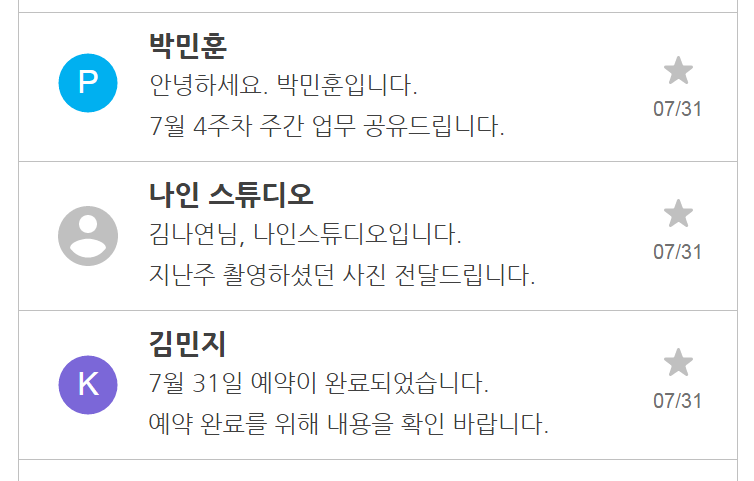
\includegraphics[scale=0.65]{favorite_sample}

사용자는 하나씩 천천히 선택/해제를 하지 않기 때문에, UI를 Blocking하지 않기 위해서 별도의 스레드에서 DB 반영을 하기로 했다.
그런데 사용자는 선택/해제를 마구 바꾸기도 하는데, 이 때문에 좀 더 세심한 처리가 필요하다.
만일 체크 상태가 바뀔 때마다 스레드를 생성하거나 스레드 풀에서 스레드를 가져다가 DB에 반영하면 어떤 일이 벌어질까? 스레드 실행은 start()를 실행한 순서대로 되지 않기 때문에 선택$\rightarrow$해제$\rightarrow$선택을 했지만, DB에 반영할 때는 선택$\rightarrow$선택$\rightarrow$해제 순으로 반영하여 최종 결과를 잘못 반영할 가능성이 있다. 
즉 실행 순서를 순차적으로 맞추어야 하는데, 바로 HandlerThread가 필요한 지점이다.\footnote{허니콤 이후의 AsyncTask도 순차 실행이 기본 동작이지만, AsyncTask는 백그라운드 스레드와 UI 스레드를 구분하고 데이터를 전달하는 목적에 더 적합하다.}
HandlerThread를 쓰지 않고서 비슷한 동작을 하려면, 백그라운드 스레드에서 무한루프를 만들고 BlockingQueue를 매개로 하여 백그라운드 스레드에서는 take를 실행하고 외부에서는 put을 실행하는 형태를 만들어야 한다.
BlockingQueue API 문서에 관련 샘플이 있는데, HandlerThread를 사용하면 구조보다 Message에 더 집중할 수 있다.\\

아래 코드를 한번 보자. 아직 버그가 있는 버전이고 이 버그를 통해 HandlerThread의 구조를 더 잘 이해할 수 있을 것이다.
\begin{lstlisting}[frame=single, caption=HandlerThread 사용 예제(버그 존재), label=src:HandlerThreadSample] 
 	private Handler favoriteHandler;
    private Looper favoriteLooper;

    @Override
    public void onCreate(Bundle savedInstanceState) {
       	... 
       	HandlerThread handlerThread 
       		= new HandlerThread("Favorite Processing Thread");
        handlerThread.start(); // (1)
        favoriteLooper = handlerThread.getLooper(); // (2)
        favoriteHandler = new Handler(favoriteLooper) {

            @Override
            public void handleMessage(Message msg) { // (3)
                MessageFavorite messageFavorite 
                		= (MessageFavorite) msg.obj;
                favoriteDao.updateMessageFavorite(messageFavorite.id, 
                		messageFavorite.favorite);
            }

        };
        
	}

	private class MessageAdapter extends ArrayAdapter<Message> {
		
		@Override
        public View getView(int position, View convertView, 
        			ViewGroup parent) {	
        		....
			holder.favorite.setOnClickListener(new View.OnClickListener() {

                @Override
                public void onClick(View view) {
                    boolean checked = ((CheckBox) view).isChecked();
                    Message message = favoriteHandler.obtainMessage();
                    message.obj = new MessageFavorite(item.id, checked);
                    favoriteHandler.sendMessage(message); // (4)
                }

            });
	}
	
	
	@Override
    protected void onDestroy() {
        if (favoriteLooper != null) {
            favoriteLooper.quit(); // (5)
        }
        super.onDestroy();
    }
\end{lstlisting}

여기서 라인별로 주요한 내용들을 얘기해보자.
\begin{itemize}
\item 9라인(1)에서 HandlerThread를 시작하였다. HandlerThread는 Thread를 상속한 것이라는 걸 기억하자.
\item 10라인(2)에서 Handler를 생성하면서 HandlerThread에서 만든 Looper를 전달하였다.
\item 38라인(4)에서 체크박스를 선택/해제할 때마다 Handler에 Message를 보낸다.
\item 14라인(3)에서 Message를 받아서 DB에 반영한다.
\item 48라인(5)에서 Looper를 종료한다. 
\end{itemize}

작동방식이 그리 어려워 보이진 않는다.
그런데 Looper를 종료할 때 null 체크를 하는 부분은 어째서일까? 
테스트를 여러 번 하다보니 NullPointerException이 발생했는데, 재현도 쉽지 않았던 부분이다. 
Thread에서 start()를 실행하면, 스레드가 바로 시작하는 것이 아니라 스케줄링에 따라 시간차가 있다. 
즉 onCreate() 실행 중에 시작할 수도 있지만, onCreate()가 끝난 이후에도 곧바로 시작한다는 보장도 없다.
이제 메인 스레드 쪽을 보면 onDestory()가 곧바로 불리는 상황이 있다. 
Activity의 onCreate() 안에서 전달된 Intent 파라미터가 유효하지 않을 때 finish()를 호출하는 경우도 있고, onStart(), onResume()에서도 마찬가지다. 
onResume() 메서드까지 어쨌든 실행했는데, 사용자가 ``왜 이리 늦지'' 하면서 Back 키를 누를 수도 있다. Back 키도 디폴트로 finish()를 호출하고, 
finish()를 통해서 onDestroy() 메서드가 호출되는데, onDestory() 실행 이전에 HandlerThread가 시작됐을 거라는 걸 보장할 수가 없다!
보통 때는 잘 되다가 드물게 NullPointerException이 발생하는 원인이 이것인데, null 체크를 하는 수 밖에 없었다.
그런데 엄밀하게 얘기하면 코드 \ref{src:HandlerThreadSample}도 정확한 코드가 아니다. 
`실행해보니 문제가 생기네' 하면서 시행착오를 넘어간 것 뿐이다.\\

이제 Looper를 제대로 종료하는 방법을 알아보자. 코드 \ref{src:HandlerThreadSample}에는 아직 오류가 있는 것일까?
문제 제기 내용은 2가지이다.\\

\underline{\bfseries 1) Looper.quit()을 쓰는 게 적절한가?}\\
DB 반영 내용이 많아서 시간이 걸린다고 가정해보자. 
사용자가 액션을 빈번하게 보냈을 때 곧바로 처리가 되지 않은 상태에서 Back 키로 종료하면, Looper.quit()에서 아직 처리하지 않은 메시지는 어떻게 하는가?
코드 \ref{src:HandlerThreadSample}에서는 Delayed Message가 없으니까, 굳이 quitSafely()가 아닌 quit()으로 종료해도 문제가 없긴 하다.\\

\underline{\bfseries 2) Looper를 null 체크하는 시점 이후에 스레드가 시작되면 어떻게 되는가?}\\
바로 타이밍 문제가 생긴다. 
Looper.loop() 메소드는 무한 루프 상태이고 스레드는 그 스레드를 시작한 Activity를 참조하고 있으므로, onDestroy() 이후에도 Activity는 내내 GC가 안 되는 문제가 발생한다.
quit()이나 quitSafely()를 호출해야만 GC 문제가 생기지 않는다.
null 체크를 해도 안 되고 안 해도 문제인 상황에 다른 해법이 있을까?
바로 한 가지가 있다.\\

MessageQueue.IdleHandler API 문서를 보면 Message를 모두 처리하고서 휴식 상태일 때 IdleHandler 인터페이스를 가지고서 할 일을 지정할 수 있다.
인터페이스의 유일한 메서드인 queueIdle()은, IdleHandler를 계속 사용하려면 true를 리턴하고 아니면 false를 리턴한다. 즉 false를 리턴하면 idle 상태가 될 때마다 queueIdle() 메서드가 실행된다.
결론적으로 IdleHandler를 등록해서 Activity가 종료되고 모든 Message가 처리되어서 idle 상태가 되었을 때 Looper.quit()을 실행하면 된다.\\

코드 \ref{src:HandlerThreadSample}과 달라지는 부분은 두 군데이다.
\begin{itemize}
\item onDestroy()에서 Looper.quit()을 실행하지 않는다.
\item MessageQueue에 IdleHandler을 등록해서 IdleHandler 안에서 Looper.quit()을 실행한다.
\end{itemize}

달라지는 부분 위주로 코드를 보자.
\begin{lstlisting}[frame=single, caption=Handler 스레드 사용 예제(Fixed), label=src:HandlerThreadSample2] 
 	@Override
    public void onCreate(Bundle savedInstanceState) {
    		....
        HandlerThread handlerThread
                = new HandlerThread("Favorite Processing Thread") {

            @Override
            protected void onLooperPrepared() { // (1)
                getLooper().myQueue().addIdleHandler(
                			new MessageQueue.IdleHandler() {

                    @Override
                    public boolean queueIdle() {
                        if (isFinishing()) { // (2)
                            getLooper().quit();
                            return false;
                        }
                        return true;
                    }

                });
            }

        };
        handlerThread.start();
        ....
	}
	
	@Override
    protected void onDestroy() {
        super.onDestroy();
    }
\end{lstlisting}

\begin{itemize}
\item 8라인(1)에 onLooperPrepared() 메서드 안에서 IdleHandler를 등록한다. onLooperPrepared() 메서드는 HandlerThread에서 일종의 hook 메서드로 Looper.prepare()가 실행된 다음에 호출된다.
\item 14라인(2)에서 isFinishing() 메서드로 종료 여부를 체크한다. isFinishing() == true인 경우에는 Looper를 종료하고, IdleHandler를 더 쓸 필요가 없으므로 queueIdle() 메서드는 false를 리턴한다.
\end{itemize}

\begin{comment}    
% 이 경우는 Thread 안에서 Handler를 쓰는 것이 낫다.
서버에서 데이터를 가져와서  로컬 데이터베이스에 넣는데 카테고리와 상세를 각각 가져온다고 하자.
카테고리가 먼저 입력되어야만 Foreign Key Contraint 문제가 발생하지 않는데, 각각 스레드로 병렬 실행한다면 상세 데이터를 먼저 가져와서 문제가 발생할 수 있다. 이런 경우에 순차 입력을 위해서 HandlerThread를 고려해보자.\\

라이브러리를 사용하면서 순차적으로 작업들을 실행할 때도 있다. 이때 하나가 끝나면 Listener에서 다음 작업을 실행하도록 만들거나, 만들어진 것을 본 적이 있을 것이다. 이런 경우도 HandlerThread를 사용하고 도중에 실패한 경우에는 HandlerThread의 quit 메서드를 호출한다.
\end{comment}

\section{스레드 풀}
\subsection{ThreadPoolExecutor}
스레드를 만들려면 Thread를 상속하거나 Thread(Runnable) 생성자에 Runnable 을 넘기는 방법이 있다. 그리고 또 한 가지는 스레드 풀을 사용하는 방법도 있다.
스레드 풀은 대기 상태의 스레드를 유지해서 태스크 실행 오버헤드를 줄임으로써 많은 개수의 비동기 작업을 실행할 때 퍼포먼스를 향상시킨다. 
그리고 스레드를 포함한 리소스를 제한하고 관리하는 방법도 제공한다. 
컴포넌트에 작업이 계속 들어온다면 스레드 풀 사용을 고려해보자. AsyncTask도 내부적으로 스레드 풀을 사용하고 있다.\\

ThreadPoolExecutor에는 4개의 생성자가 있는데 ThreadFactory가 빠져있는 세 번째 생성자 위주로 보자.\\

ThreadPoolExecutor(int corePoolSize, int maximumPoolSize, long keepAliveTime, TimeUnit unit,\\ BlockingQueue<Runnable> workQueue, RejectedExecutionHandler handler)\\

파라미터 가운데서 corePoolSize나 maximumPoolSize는 이름만으로 이해될 것이다. 
pool의 스레드 개수가 coreSize보다 커진다면, 초과하는 개수만큼의 작업은 끝나고 나서는 스레드를 유지할 필요는 없다. 
조금 혼동되는 부분이 ThreadPoolExecutor 생성자에서 corePoolSize만큼 미리 생성하는가 하면 그렇지는 않다. 해당 용도의  prestartCoreThread() 메서드는 별도로 존재한다. 기본적으로 execute()나 submit()을 호출하는 순간에 실행중인 스레드 개수가 corePoolSize보다 적으면 새로 스레드를 추가하는 형태이다.
keepAliveTime과 unit은 이때 바로 제거하지 않고 대기하는 시간이다. 보통 unit에는 TimeUnit.MINUTES나 TimeUnit.SECONDS를 사용한다.
workQueue도 내용상 중요하다. pool에서는 corePoolSize 개수만큼 유지하려 하고 추가로 요청이 들어오면 workQueue에 쌓는다. 이 workQueue 개수 제한이 넘으면 pool의 스레드 개수를 늘리는 것을 고려해야 한다. workQueue에 쓸 수 있는 것은 세 가지이다.
\begin{itemize}
\item ArrayBlockingQueue: Queue 개수 제한이 있으며 요청이 들어오면 일단 Queue에 쌓는다. Queue가 꽉 차서 더 넣을 수 없는 경우에는 maximumPoolSize가 될 때까지 스레드를 하나씩 추가해서 사용한다
\item LinkedBlockingQueue: 일반적으로 Queue 개수에 제한이 없다. 들어오는 요청마다 계속해서 쌓는데 이 경우에는 maximumPoolSize가 의미가 없다. LinkedBlockingQueue도 LinkedBlockingQueue(int capacity) 생성자를 사용해서 Queue 개수에 제한을 둘 수는 있다.
\item SynchronousQueue: 요청을 쌓지 않고 바로 준비된 스레드로 처리한다. 결국 Queue를 안 쓴다는 의미이다.
모든 스레드가 작업중이라면 maximumPoolSize까지는 스레드를 생성해서 처리한다. 
\end{itemize}

ThreadPoolExecutor가 shutdown되거나, 최대 스레드 개수와 workQueue 용량을 초과할 때는 때는 태스크가 거부된다. 거부되는 방식을 정하는 것이 ThreadPoolExecutor 생성자의 마지막 파라미터인 RejectedExecutionHandler이고 미리 정의된 4개가 있다.
\begin{itemize}
\item ThreadPoolExecutor.AbortPolicy: 디폴트 handler로 RejectedExecutionException 런타임 예외를 발생시킨다.
\item ThreadPoolExecutor.CallerRunsPolicy: 스레드를 생성하지 않고 요청 태스크를 호출하는 스레드에서 바로 실행된다. 
\item ThreadPoolExecutor.DiscardPolicy: 요청 태스크가 조용히 제거된다.
\item ThreadPoolExecutor.DiscardOldestPolicy: workQueue에서 가장 오래된 태스크를 제거한다.
\end{itemize}

AsyncTask.THREAD\_POOL\_EXECUTOR도 RejectedExecutionHandler를 따로 넣지 않아서 기본으로 AbortPolicy가 적용된다. AsyncTask는 기존에는 maximumPoolSize = 128개와 workQueue 개수 = 10으로 지정되어 있었고, 킷캣부터 maximumPoolSize = (CPU 개수 * 2 + 1)과 workQueue 개수 = 128로 변경되었는데, 어쨌든 maximumPoolSize + workQueue 개수를 넘으면 에러가 발생한다. 파일 사이즈가 큰 이미지들을 AsyncTask를 이용해서 한꺼번에 다운로드한다면 발생 케이스를 재현해볼 수 있다.\\

앱에서 ThreadPoolExecutor를 사용할 때는 가장 쓸모 있는 RejectedExecutionHandler는 DiscardOldestPolicy이다. 
화면에서 계속 스크롤하거나 다른 화면으로 이동할 때, 지금 보여지는 화면이 중요하고 이미 지나가버린 것은 상대적으로 중요하지 않다. 
DiscardOldestPolicy를 사용하면 오래된 것을 workQueue에서 제거하고 최신의 태스크를 workQueue에 추가한다. 
아래 샘플은 ImageView에 표시할 이미지 파일을 다운로드해서 보여줄 때, DiscardOldestPolicy를 사용한 예이다.
ListView의 각 아이템에 ImageView가 있을 때, 현재 스크롤된 위치에서 ImageView의 url이 workQueue의 마지막에 들어가고 workQueue 사이즈를 초과하는 경우 스크롤된 지 오래된 ImageView의 url은 제거된다.
\begin{lstlisting}[frame=single] 
	private static final int FIXED_THREAD_SIZE = 4;
	private static final int QUEUE_SIZE = 20;
	
	private ThreadPoolExecutor executor
		= new ThreadPoolExecutor(FIXED_THREAD_SIZE, FIXED_THREAD_SIZE, 
				0L, TimeUnit.MILLISECONDS, 
				new LinkedBlockingQueue<Runnable>(QUEUE_SIZE), 
				new ThreadPoolExecutor.DiscardOldestPolicy());
	
	private void queueDownload(ImageView imageView, String url) {
		executor.submit(new ImageDownloadTask(imageView, url));
	}
\end{lstlisting}
스레드 개수는 4개를 쓰고 workQueue 사이즈는 20개이므로, 동시에 24개까지는 태스크를 집어넣을 수 있다. 그 이상으로 submit()을 실행하면 workQueue에서 오래된 태스크를 제거하고서 새로운 태스크를 workQueue에 추가한다.\\
	
\subsection{ScheduledThreadPoolExecutor}
지연/반복 작업에 대해서는 ScheduledThreadPoolExecutor를 사용할 수 있다.
앞에서 Handler를 이용해도 지연/반복 작업을 할 수 있다고 했는데, 화면 갱신이라면 Handler를 쓰는 게 적절하지만 네트워크 통신이나 DB 작업 같은 것이 지연/반복 실행되는 경우는 ScheduledThreadPoolExecutor를 고려하자.\\

다른 옵션으로 Timer를 생각할 수도 있지만 Timer API 문서를 보면 Timer보다는 ScheduledThreadPoolExecutor를 사용하도록 권장한다. Timer는 실시간 태스크 스케줄링을 보장하지 않고(스레드를 하나만 생성해서 사용하기 때문에 앞서 실행되는 작업 때문에 예정 시간에 맞지 않게 실행될 수 있다), 여러 스레드가 동기화 없이 하나의 타이머를 공유하는 문제가 있다.\footnote{자바 병렬 프로그래밍 6.2.5에 관련해서 상세한 내용이 나와있다.}\\

ScheduledThreadPoolExecutor도 ThreadPoolExecutor와 마찬가지로 4개의 생성자가 있는데, ThreadPoolExecutor에 있는 maximumPoolSize, keepAliveTime, unit, workQueue 4개의 파라미터가 빠져 있다. 
이 4개는 ScheduledThreadPoolExecutor에서 고정되어 있는데,
maximumPoolSize = Integer.MAX\_VALUE, keepAliveTime = 0, workQueue에는 내부 클래스인 DelayWorkQueue 인스턴스가 전달된다.
DelayWorkQueue는 기본 사이즈는 16인데, 들어오는 게 많아지면 계속 사이즈가 커지고 제한이 없다.\\

ScheduledThreadPoolExecutor의 사용 예는 \ref{subsec:messenger}절에서 볼 수 있다.

\begin{comment}
public ScheduledFuture<?> schedule (Runnable command, long delay, TimeUnit unit)
public ScheduledFuture<V> schedule (Callable<V> callable, long delay, TimeUnit unit)
public ScheduledFuture<?> scheduleAtFixedRate (Runnable command, long initialDelay, long period, TimeUnit unit)
public ScheduledFuture<?> scheduleWithFixedDelay (Runnable command, long initialDelay, long delay, TimeUnit unit)
\end{comment}

\subsection{Executors}
ThreadPoolExecutor, ScheduledThreadPoolExecutor는 직접 생성하는 것보다는 Executors의 팩토리 메서드로 생성하는 경우가 많다.
Executors에서 리턴하는 ExecutorService, ScheduledExecutorService는 ThreadPoolExecutor, ScheduledThreadPoolExecutor의 상위 인터페이스이다.\\

Executors의 주요 팩토리 메서드는 아래와 같다.
\begin{itemize}

\item newFixedThreadPool(int nThreads): 파라미터로 전달되는 고정 개수까지 스레드를 생성한다. workQueue는 개수 제한이 없다.
\begin{verbatim}
new ThreadPoolExecutor(nThreads, nThreads, 0L, TimeUnit.MILLISECONDS, 
    new LinkedBlockingQueue<Runnable>())
\end{verbatim}

\item newCachedThreadPool(): 필요할 때 스레드를 생성하고 스레드의 개수는 제한이 없다. keepAliveTime이 60초로 길다는 것이 특징이다. 이 때문에 Cached라는 수식어가 붙었다.
\begin{verbatim}
new ThreadPoolExecutor(0, Integer.MAX_VALUE, 60L, TimeUnit.SECONDS, 
    new SynchronousQueue<Runnable>());
\end{verbatim}

\item newSingleThreadExecutor(): 단일 스레드를 사용해서 순차적으로 처리한다. workQueue는 개수 제한이 없다. 
\begin{verbatim}
new FinalizableDelegatedExecutorService
	(new ThreadPoolExecutor(1, 1, 0L, TimeUnit.MILLISECONDS, new LinkedBlockingQueue<Runnable>())
\end{verbatim}
newFixedThreadPool(1)과 동일한 결과를 리턴하는 것으로 보이는데, 다시 FinalizableDelegatedExecutorService로 Wrapping하였다. Wrapping의 효과는 스레드 개수를 1이 아닌 다른 값으로 변경하지 못하게 하는 것이다. 단순히 newFixedThreadPool(1)로 리턴된 것은 ThreadPoolExecutor로 캐스팅해서 setCorePoolSize()나 setMaximumPoolSize() 메서드로 스레드 개수를 변경할 수 있다.

\item newScheduledThreadPool(int corePoolSize): corePoolSize 개수의 ScheduledThreadPoolExecutor를 만든다.
\begin{verbatim}
new ScheduledThreadPoolExecutor(corePoolSize)
\end{verbatim}

\end{itemize}

팩토리 메서드 가운데서 용도에 맞는 게 없다면 결국 ThreadPoolExecutor, ScheduledThreadPoolExecutor를 직접 사용해야만 한다.\\

\section{AsyncTask}
\label{sec:asynctask}
동시성 프로그래밍에 익숙하지 않은 경우에는 안드로이드 API에 과도하게 의존하는 경우도 있다.
예를 들어, Service에서 시간이 오래 걸리는 작업이라면 단순하게 스레드를 생성해서 실행하면 되는데, AsyncTask를 생성해서 doInBackground() 메서드만을 구현하는 케이스도 볼 수 있다. 
AsyncTask는 백그라운드 스레드에서 작업하는 진행 상태나 결과 데이터를 UI 스레드에 전달하고, 백그라운드 스레드와 UI 스레드를 고민하지 않고 구분해서 쓸 수 있도록 만들어진 것이다.
AsyncTask는 onPostExecute() 오버라이드가 필요하지 않을 때는, 즉 UI 작업이 필요하지 않는 경우 쓰지 않는 게 좋다. 이때는 AsyncTask의 스레드 풀을 사용하는 것뿐이다.

백그라운드 스레드와 UI 스레드를 구분해서 사용하는 여러 방법을 살펴보자.
\begin{lstlisting}[frame=single] 
	public void onClick(View v) {
    	new Thread(new Runnable() {
    		
    		@Override
        	public void run() {
            	Bitmap b = loadImageFromNetwork("http://example.com/image.png");
            	mImageView.setImageBitmap(b);
        	}
        	
    	}).start();
	}
\end{lstlisting}
백그라운드 스레드에서 UI를 변경하므로 CalledFromWrongThreadException이 발생한다.
이를 해결하는 방법은 앞에서도 얘기했듯이 여러 버전이 있다.

\begin{enumerate}
\item Handler 이용(2가지 방식)
\begin{lstlisting}[frame=single]
	private final static int BITMAP_MSG = 1;
	
	private Handler mHandler = new Handler() {
		
		@Override
		public void handleMessage(Message msg) {
			if (msg.what == BITMAP_MSG) {
				mImageView.setImageBitmap((Bitmap) msg.obj);
			}
		}
		
	};
	
	public void onClick(View v) {
    	new Thread(new Runnable() {
    		
    		@Override
        	public void run() {
            	final Bitmap bitmap = loadImageFromNetwork("http://example.com/image.png");
            	Message message = Message.obtain(mHandler, BITMAP_MSG, bitmap);
            	mHandler.sendMessage(message);
        	}

	
    	}).start();
	}
\end{lstlisting}

\begin{lstlisting}[frame=single]
	private Handler mHandler = new Handler();
	
	public void onClick(View v) {
    	new Thread(new Runnable() {
    	
    		@Override
        	public void run() {
            	final Bitmap bitmap = loadImageFromNetwork("http://example.com/image.png");
            	mHandler.post(new Runnable() {
            		
                	public void run() {
                    	mImageView.setImageBitmap(bitmap);
                	}
                	
            	});
        	}

	
    	}).start();
	}
\end{lstlisting}

\item View의 post() 메서드에 Runnable 전달: 내부적으로 Handler를 사용한다. Activity의 runOnUiThread() 메서드도 동일한 형태로 사용하면 된다.
\begin{lstlisting}[frame=single] 
	public void onClick(View v) {
    	new Thread(new Runnable() {
    	
    		@Override
        	public void run() {
            	final Bitmap bitmap =
                    loadImageFromNetwork("http://example.com/image.png");
            	mImageView.post(new Runnable() {
                	public void run() {
                    	mImageView.setImageBitmap(bitmap);
                	}
            	});
        	}
        	
    	}).start();
	}
\end{lstlisting}
	
\item AsyncTask 이용: 내부적으로 Handler를 이용한 첫 번째 방식으로 되어있다.
\begin{lstlisting}[frame=single]
	public void onClick(View v) {
    	new DownloadImageTask().execute("http://example.com/image.png");
	}

	private class DownloadImageTask extends AsyncTask<String, Void, Bitmap> {
	
		@Override
    	protected Bitmap doInBackground(String... urls) {
        	return loadImageFromNetwork(urls[0]);
    	}

      	@Override
    	protected void onPostExecute(Bitmap result) {
        	mImageView.setImageBitmap(result);
    	}
    	
	}	
\end{lstlisting}
\end{enumerate}
여기 샘플에서 빠진 부분이 있다. 바로 loadImageFromNetwork() 메서드에 대한 예외 처리가 없는데 이 내용은 뒤에서 이슈로 살펴보겠다.\\

AsyncTask는 제네릭 클래스이고 타입 파라미터에는 Params, Progress, Result 세 가지가 있다. 진행 상태가 필요하지 않은 경우 Progress에 Void가 들어가는 경우는 있지만 모두 다 Void인 것도 권장되는 형태는 아니다.\\

아래는 개발자 가이드에 있는 내용이다.
\begin{lstlisting}[frame=single]
private class MyTask extends AsyncTask<Void, Void, Void> { ... }
\end{lstlisting}
이것은 백그라운드 스레드와 UI 스레드를 구분하기 위한 용도로만 쓰이는 것으로 Handler를 이용하는 게 더 단순할 수 있다.\\

AsyncTask는 안드로이드 개발자에게는 익숙한 것이기 때문에 이 절에서는 이슈 중심으로 살펴보자.

\subsection{병렬 실행 시 실행 순서}
안드로이드 버전이 올라가면서 많은 논란이 있던 내용 가운데 하나가 AsyncTask를 실행할 때 기본 동작이 `병렬 실행'에서 `순차 실행'으로 바뀐 것이다. 
병렬 실행이 여러 문제를 일으켰기 때문에, 제어 가능하다고 자신하는 경우에만 `동시 실행'을 쓰라는 의미이다.
그럼에도 여전히 AsyncTask는 병렬 실행을 기본으로 해서 개발할 때가 많다.\\

AsyncTask의 병렬 실행이 필요한 경우를 들어보자. 
화면에 여러 가지 정보를 보여주는 데 DB나 서버 API로 단번에 가져오지 못하는 경우가 많다. 도착 지점의 날씨 정보와 주변 주차장 정보를 화면에 보여주고 싶은데 서버 API가 따로라면 API를 병렬로 호출하는 게 유리할 것이다.\\

2개 이상을 동시에 실행하는 경우도 있겠지만 일단 2개로 제한해서 얘기를 진행하자.   
2개의 AsyncTask를 시작하면 메인 스레드에서 동작하는 onPostExecute()는 단일 스레드 규칙에 의해 하나씩 실행이 되지만 2개의 AsyncTask 가운데 어느 것이 먼저 doInBackground()를 먼저 끝내고 onPostExecute()를 실행할 지는 알 수 없다. 
예를 들어, 필자는 동일한 데이터 구조를 로컬에서 가져온 것과 API를 통해 서버에서 가져온 것을 조합해서 화면에 보여준 적이 있다. 
2개를 각각 AsyncTask로 만들고 로컬 데이터를 가져오는 것을 먼저 시작하고(AsyncTaskA) 서버 데이터를 가져오는 것을 바로 다음에 시작하였다(AsyncTaskB). 
로컬 데이터가 결과를 빨리 가져온다는 가정하에 AsyncTaskA에서는 멤버 변수에 데이터만 저장하고 AsyncTaskB의 onPostExecute()에서 조합해서 화면을 보여주었다.
결과는 어땠을까? 아주 드물지만 로컬 데이터를 먼저 가져온다는 가정이 어긋나는 경우가 생겨서 에러를 발생시켰다. 
작업량이 많고 적은 것으로 판단하면 안 된다.
백그라운드 스레드 간에는 무엇이 먼저 실행된다고 가정하면 안 된다. 극단적으로 말하면 동작이 운에 따른 것이 된다.
이런 문제가 제어가 어렵다면 차라리 `순차 실행'을 하는 게 나을 수도 있다.\\

일반적으로 2개의 AsyncTask 간에 병렬 실행도 하면서 결과를 합해야 하는 경우에는 2가지 정도 방법을 사용한다.
\begin{itemize}
\item 멤버 변수에 비트합을 사용한다. 2개의 AsyncTask가 끝나면 각각 비트를 합하고 둘 다 충족했다면 onPostExcecute() 메서드에서 데이터를 조합해서 보여준다. 예외가 나오는 케이스도 고려해야만 한다. 
\item CountDownLatch를 이용해서 AsyncTask 간에 다른 한 쪽의 작업이 끝날 때까지 대기했다가 이후에 데이터를 조합한다. 이 방식은 \url{http://suribada.com/wp/?p=13}을 참고하자.
\end{itemize}

AsyncTask의 대안으로 RxJava 라이브러리를 사용하기도 한다. RxJava에 대한 내용은 \url{https://github.com/ReactiveX/RxJava/wiki}를 참고하자.

\subsection{Activity 종료 시점과 불일치}
Activity에서 AsyncTask의 백그라운드 작업 실행 도중에 Back 키를 통해서 Activity를 종료하면 AsyncTask는 어떻게 되는가? 메모리에는 Activity가 남아있어서 onPostExecute()도 정상적으로 실행되고 그 안에서 setText()와 같은 UI 변경 메서드도 잘 실행된다. 다만 눈앞에서 사라져서 보이지 않을 뿐이다.
이렇게 Activity 종료 시점과 AsyncTask가 끝나는 시점이 달라서 발생하는 문제가 몇 가지 있다.\\

\begin{itemize}
\item 메모리 문제가 발생할 수 있다. Activity가 Back 키로 종료할 때는 AsyncTask가 오래 걸리는 게 아니라면 큰 문제까지는 아니다. 
AsyncTask 때문에 문제가 생기는 것은 화면 회전으로 인해 계속해서 AsyncTask가 쌓여서 실행하는 경우이다.
Activity가 화면 방향 고정이거나 android:configChanges 속성에 ``orientation''이 들어있지 않은 경우 화면 회전 시마다 Activity는 종료되고 새로 시작되는데 새로 시작되는 것은 다른 인스턴스이다. 
AsyncTask가 아직 실행 중인 경우에는 기존 Activity도 메모리에서 제거되지 않는다. 빈번하게 화면을 회전할 때 OutOfMemoryError가 발생하는 원인 가운데 하나가 될 수 있다.
`안드로이드 멀티스레딩' 책에서 제안한 방법은 Activity를 WeakReference로 한 정적 내부 클래스로 AsyncTask를 만드는 것인데, 번거로워서 쓰기에 망설여진다. Activity가 종료될 때 AsyncTask를 함께 종료하는 방법을 찾아보는 게 좋겠다. 이에 대해서는 바로 다음 절에서 살펴보자.  
또 다른 대안으로는 Loader 프레임워크를 사용하는 방법도 있다. Loader 사용은 복잡하지만 충분히 고려할 만하다.\footnote{\url{http://developer.android.com/intl/ko/guide/components/loaders.html} 내용을 참고하자.}

\item AsyncTask를 순차 실행한다면(SERIAL\_EXECUTOR) 화면 회전 시마다 작업이 쌓이므로 갈수록 실행이 느려질 수 있다.

\item Fragment에서 AsyncTask를 실행할 때 문제가 발생할 수 있다. AsyncTask 실행 도중에 Back 키로 Activity를 종료하면 Fragment는 Activity와 분리되면서 Fragment에서 getActivity()는 null을 리턴한다. AsyncTask의 onPostExecute()에서 Context를 사용할 때 NullPointerException이 발생하므로, 권장되는 방식은 onPostExecute() 메서드 시작 부분에서 getActivity() == null을 체크해서 리턴하는 것이다. 어차피 화면이 없으므로 UI를 업데이트하지 않고 리턴하는 것이 적절하다. 
\end{itemize}

\subsection{AsyncTask 취소}
AsyncTask에는 cancel() 메서드가 있다. 이 메소드는 AsyncTask의 mCancelled 변수를 true로 만들고, 이로 인해 스레드 작업 이후에 onPostExecute() 대신 onCancelled()가 불린다. 스레드 작업이 오래 걸리는 경우에 doInBackground() 메서드에서는 중간에 isCancelled() 메서드로 체크해서 바로 리턴하는 로직을 쓰는 것을 권장하고 있다. 무엇을 리턴하든 간에 onPostExeceute()는 불리지 않고 onCancelled()에서 처리한다.\footnote{허니콤부터 onCancelled() 메서드는 파라미터가 없는 버전에 doInBackground()의 결과를 전달하는 onCancelled(Result result) 메서드가 추가되었다.}\\

결론적으로 AsyncTask를 Activity 종료 시점에 근접하게 종료하는 방법은 isCancelled() 메서드를 doInBackground()에서 곳곳에 사용하고(특히 루프문에서), AsyncTask를 멤버 변수로 유지하고서 Activity의 onDestroy()에서 AsyncTask의 cancel() 메서드를 호출하는 것이다.\\

%mayInterruptIfRunning 파라미터에 true를 전달하면 무엇이 다를까? 이것은 스레드에 인터럽트 신호를 보내는 것으로 스레드가 바로 종료하는 것은 아니다.
% 사용하는 클래스에서 사용?(예로 소켓 종료)
% sleep 샘플(sleep 문제...)

\subsection{예외 처리 메서드 부재} 
AsyncTask에는 정상적인 데이터 처리를 위한 onPostExcecute()와 작업 취소를 위한 onCancelled() 메서드는 있는데 예외 처리를 위한 onError() 메서드는 없다. 
백그라운드 스레드에서 하는 작업은 네트워크 문제와 같은 다양한 예외 케이스가 있어서, 이 경우에는 문제가 발생했다고 화면에 표시하는 경우가 많다. 즉 예외 케이스에도 UI 작업이 필요한 것이다.\\

백그라운드 스레드와 UI 스레드를 분리할 때 예외에 대해서도 고려가 필요한데, 이 내용이 AsyncTask에서 빠져서 AsyncTask의 기본 형태를 변형해서 사용하는 경우가 생겼다.
\begin{lstlisting}[frame=single]
	public void onClick(View v) {
    	new DownloadImageTask().execute("http://example.com/image.png");
	}

	private class DownloadImageTask extends AsyncTask<String, Void, Bitmap> {
	
		@Override
    	protected Bitmap doInBackground(String... urls) {
    		try {
        		return loadImageFromNetwork(urls[0]);
        	} catch (Exception e) {
        		return null; // (1)
        	}
    	}

      	@Override
    	protected void onPostExecute(Bitmap result) {
    		if (result == null) { // (2)
    			// show error message at UI
    			return;
    		}
        	mImageView.setImageBitmap(result);
    	}
    	
	}	
\end{lstlisting}
예외가 발생할 때 12라인(1)에서 null을 리턴하고 18라인(2)에서 체크해서 null이면 에러 메시지를 보여주는 식이다. 이 방식도 문제가 완전히 해결된 것은 아니다. 
loadImageFromNetwork()에서 예외는 발생하지 않지만 null을 리턴하는 경우가 있다면, error message가 의도에 맞지 않는다. 예외 상황이 아니면 null이 나올 수 없도록 하거나, 어쨌든 null이 나오는 것을 문제로 간주한다면 가능한 방식이다. 

\begin{lstlisting}[frame=single]
	public void onClick(View v) {
    	new DownloadImageTask().execute("http://example.com/image.png");
	}

	private class DownloadImageTask extends AsyncTask<String, Void, Boolean> {
	
		private Bitmap bitmap;
		
		@Override
    	protected Bitmap doInBackground(String... urls) {
        	try {
        		bitmap = loadImageFromNetwork(urls[0]);
        		return Boolean.TRUE;
        	} catch (Exception e) {
        		return Boolean.FALSE;
        	}
    	}

      	@Override
    	protected void onPostExecute(Boolean result) {
    		if (!result) {
    			// show error message
    			return;
    		}
        	mImageView.setImageBitmap(bitmap);
    	}
    	
	}	
\end{lstlisting}
원래 의도와는 다르게 결과값을 doInBackground()에서 onPostExecute()로 전달하는 것이 아니고,  성공 여부를 Boolean 값을 리턴해서 전달하고 있다. 
전달하고자 하는 결과값은 뜬금없이 AsyncTask의 멤버 변수에 대입돼서 onPostExecute()에서 사용한다.
가능은 하지만 원래 AsyncTask의 사용 방식과 차이가 생긴다.\\
%3가지 패턴(Handler, tuple, 멤버 변수, true, false)

군더더기 코드가 생겨나는데 이에 대한 대안으로 앞에서도 언급한 RxJava를 사용하기도 한다. RxJava에서는 예외에 대한 처리 방법을 기본으로 제공한다.
%http://www.javalobby.org/java/forums/t83677.html Interruptible Method
%http://stackoverflow.com/questions/4767553/safe-use-of-httpurlconnection
% http://www.androiddesignpatterns.com/2012/07/loaders-and-loadermanager-background.html
